\section{Literature Review}
\label{sec:lit}

% Template: develop from the previous reports and the supervisors' feedback; flow logically, not
% necessarily chronologically; end with the major work, its relevance, and the research gaps.
This section reviews the models used for multi-UAV cable-suspended transport, the centralised and
distributed control approaches, the work on changes in team composition, the execution layer and
steady-error rejection, and simulation fidelity, and ends with a comparison and the research gap
this thesis addresses.

% SUPERSEDED 12 Oct 2026: no longer input. Its content is condensed into lit_transport.tex (Section 2.1);
% fig:tension is not in the main text. Listed for deletion in docs/thesis_work_2026-10-12b.md.
% modelling.tex -- Literature review: cable models and their assumptions.
% Restructured 9 Oct (structure audit): the single-quadrotor model and fig:quad_frames are cut, the
% spring-damper equation is cut, and this thesis's own payload model moved to Source/src/model.tex
% (Methodology), merged with the planner's model. Simulation fidelity moved to Literature_review.tex.

\subsection{Cable-Suspended Transport and Model Assumptions}
\label{sec:lit_models}

The assumptions made about the cable set both the complexity of the dynamics and the validity of
the controller. The literature uses two models (Figure~\ref{fig:tension}).

\begin{figure}[h]
\centering
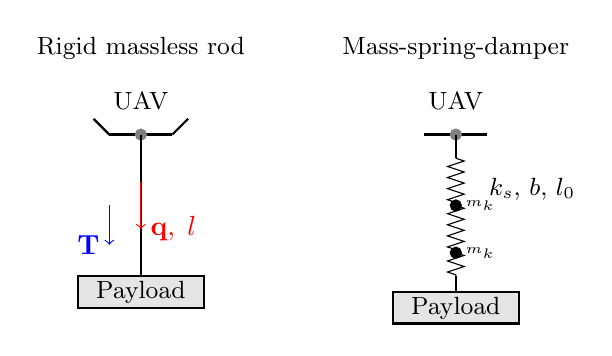
\begin{tikzpicture}[scale=1.0]
  % --- Left: Rigid rod ---
  \node[font=\small] at (-2, 3.5) {Rigid massless rod};

  % UAV
  \draw[thick] (-2.4,2.4) -- (-1.6,2.4);
  \draw[thick] (-2.4,2.4) -- (-2.6,2.6);
  \draw[thick] (-1.6,2.4) -- (-1.4,2.6);
  \filldraw[gray] (-2,2.4) circle (2pt);
  \node[above] at (-2,2.6) {\small UAV};

  % Rigid cable with unit vector label
  \draw[thick] (-2,2.4) -- (-2,0.6);
  \draw[->,red] (-2,1.8) -- (-2,1.2)
      node[right] {$\mathbf{q}, \; l$};

  % Payload
  \draw[thick,fill=gray!20] (-2.8,0.2) rectangle (-1.2,0.6);
  \node[font=\small] at (-2,0.4) {Payload};

  % Tension label
  \draw[->,blue] (-2.4,1.5) -- (-2.4,1.0)
      node[left] {$\mathbf{T}$};

  % --- Right: Spring-damper ---
  \node[font=\small] at (2, 3.5) {Mass-spring-damper};

  % UAV
  \draw[thick] (1.6,2.4) -- (2.4,2.4);
  \filldraw[gray] (2,2.4) circle (2pt);
  \node[above] at (2,2.6) {\small UAV};

  % Spring segments with lumped masses
  \draw[thick] (2,2.4) -- (2,2.1);
  \draw[decorate, decoration={zigzag,segment length=4pt, amplitude=3pt}]
      (2,2.1) -- (2,1.5);
  \filldraw (2,1.5) circle (2pt) node[right] {\tiny $m_k$};
  \draw[decorate, decoration={zigzag,segment length=4pt, amplitude=3pt}]
      (2,1.5) -- (2,0.9);
  \filldraw (2,0.9) circle (2pt) node[right] {\tiny $m_k$};
  \draw[decorate, decoration={zigzag,segment length=4pt, amplitude=3pt}]
      (2,0.9) -- (2,0.6);
  \draw[thick] (2,0.6) -- (2,0.4);

  % k_s and b labels
  \node[right, font=\small] at (2.3,1.7) {$k_s,\, b,\, l_0$};

  % Payload
  \draw[thick,fill=gray!20] (1.2,0.0) rectangle (2.8,0.4);
  \node[font=\small] at (2,0.2) {Payload};
\end{tikzpicture}
\caption{Cable modelling approaches.}
\label{fig:tension}
\end{figure}

The most common is the \textit{rigid massless rod}, adopted by \cite{efficient} and \cite{wahbaKinodynamicMotionPlanning2024}: a rigid link of fixed length $l$ along the unit vector $\mathbf{q}_i$, with the tension acting purely along it,

\begin{equation}
    \mathbf{T}_i = \lambda_i \mathbf{q}_i, \quad \lambda_i \geq 0
\end{equation}

where $\lambda_i$ is the tension, non-negative because a cable can pull but not push. The state stays compact and tractable, but slack cannot be captured.

The \textit{mass-spring-damper chain} of \cite{distributedNMPC} discretises the cable into $n$ lumped masses joined by spring--damper links of stiffness $k_s$, damping $b$ and rest length $l_0$. It captures sag and oscillation, at $6n$ extra states per cable.

Whatever the model, most controllers assume taut cables, with tension strictly positive throughout the task. A slack cable adds a unilateral constraint and a discontinuity in the equations of motion, and handling it rigorously remains open \cite{efficient}. For moderately aggressive indoor flight the rigid rod with taut cables is sufficient, consistent with \cite{tudelft}.

% control.tex -- Literature review: control architectures, changes in team composition, execution
% layer. Restructured 9 Oct (structure audit): existing.tex merged in (the TU Delft, Quan and Bacheti
% paragraphs), fig:cost_scaling cut, the RL and hybrid paragraphs cut to one sentence each, the stale
% architecture paragraph and fig:control_arch cut, the comparison moved to Literature_review.tex.

\subsection{Centralised Control}

Multi-UAV control architectures are typically classified according to their information structure and decision-making hierarchy, which directly affects scalability, robustness to communication failure, and computational burden \cite{nathanReviewAutonomousMultiagent2011}. Centralised architectures rely on a single coordinator that has global state information and computes all control actions. However, distributed and decentralised approaches allocate computation across UAVs, relying only on local communication or sensing. These differences are important in cable-suspended payload systems, where coupling through the payload induces strong dependencies between UAVs that must be either explicitly coordinated or implicitly handled through local interactions \cite{brambillaSwarmRoboticsReview2013}. Figure~\ref{fig:arch_comparison} highlights the difference in information flow and coordination structure between centralised and distributed implementations.

\begin{figure}[h]
\centering
\begin{tikzpicture}[
    node distance = 0.55cm and 0.6cm,
    box/.style     = {rectangle, rounded corners=4pt, draw, thick,
                      minimum width=2.0cm, minimum height=0.7cm,
                      font=\small, text centered},
    central/.style = {box, fill=blue!12, draw=blue!50!black},
    uav/.style     = {box, fill=orange!15, draw=orange!60!black},
    payload/.style = {box, fill=gray!18, draw=gray!60, minimum width=2.2cm},
    arrow/.style   = {-Stealth, thick},
    dasharrow/.style = {-Stealth, thick, dashed, gray},
    label/.style   = {font=\footnotesize\itshape}
]

%% LEFT PANEL — CENTRALISED
\begin{scope}
\node[central, minimum width=2.8cm, minimum height=1.0cm]
    (coord) {\textbf{Central Node}};

\node[uav, below left=0.5cm and -0.3cm of coord]  (u1l) {UAV 1};
\node[uav, below=0.5cm of coord]                  (u2l) {UAV 2};
\node[uav, below right=0.5cm and -0.3cm of coord] (u3l) {UAV 3};
\node[payload, below=0.9cm of u2l] (pl) {Payload};

\draw[<->, thick, purple!70] (coord.south west) -- ++(-0.3,0) -- (u1l.north);
\draw[<->, thick, purple!70] (coord.south)      -- (u2l.north);
\draw[<->, thick, purple!70] (coord.south east) -- ++(0.3,0) -- (u3l.north);

\draw[thick, gray!70] (u1l.south) -- (pl.north west);
\draw[thick, gray!70] (u2l.south) -- (pl.north);
\draw[thick, gray!70] (u3l.south) -- (pl.north east);

\node[above=0.25cm of coord, font=\normalsize\bfseries] (ltitle) {Centralised};

\begin{scope}[on background layer]
  \node[draw=blue!30, fill=blue!4, rounded corners=6pt, inner sep=8pt,
        fit=(ltitle)(u1l)(u3l)(pl)] {};
\end{scope}
\end{scope}

%% RIGHT PANEL — DISTRIBUTED
\begin{scope}[xshift=7.5cm]
\node[uav] (u2r) {UAV 2};
\node[uav, below left=1.1cm and 0cm of u2r]  (u1r) {UAV 1};
\node[uav, below right=1.1cm and 0cm of u2r] (u3r) {UAV 3};
\node[payload, below=2.2cm of u2r] (pr) {Payload};

\draw[<->] (u1r) -- (u2r);
\draw[<->] (u2r) -- (u3r);
\draw[<->] (u1r) -- (u3r);

\draw[thick, gray!70] (u1r.south) -- (pr.north west);
\draw[thick, gray!70] (u2r.south) -- (pr.north);
\draw[thick, gray!70] (u3r.south) -- (pr.north east);

\draw[arrow, gray!50, thin] (pr.north west) -- (u1r.south);
\draw[arrow, gray!50, thin] (pr.north)      -- (u2r.south);
\draw[arrow, gray!50, thin] (pr.north east) -- (u3r.south);

\node[above=0.25cm of u2r, font=\normalsize\bfseries] (rtitle)
    {Distributed / Decentralised};

\begin{scope}[on background layer]
  \node[draw=orange!40, fill=orange!4, rounded corners=6pt, inner sep=10pt,
        fit=(rtitle)(u1r)(u2r)(u3r)(pr)] {};
\end{scope}
\end{scope}

\end{tikzpicture}
\caption{Centralised versus distributed/decentralised control architectures.}
\label{fig:arch_comparison}
\end{figure}

In a centralised architecture, a single node receives state information from all UAVs and computes commands for the entire team. This simplifies the enforcement of global constraints such as cable tension limits, collision avoidance between UAVs, and force allocation, and is a natural fit when a single computer commands all UAVs, as is the case in this work. The primary drawbacks are that computational cost tends to grow with the number of UAVs, and the central node means a single point of failure for the system \cite{dimakosStudyCentralisedDecentralised2021}.

\subsubsection{Trajectory-Based Planning with Receding Horizon}

Several centralised methods separate the control problem into a high-level trajectory planner and a low-level tracker. Sun et al.\ \cite{tudelft}, the closest prior work and the primary performance benchmark of this thesis, adopt this structure. A centralised receding-horizon optimal control problem is solved online at 10\,Hz over the full coupled load--cable--UAV dynamics, enforcing thrust limits, cable tautness and collision avoidance directly as path constraints, and generates trajectories for each UAV and the payload. Each UAV tracks its trajectory with an onboard incremental nonlinear dynamic inversion (INDI) controller that compensates for cable forces through inertial measurements, removing the need for any sensors on the load (Section~\ref{sec:lit_execution}). Real-world experiments with three and four UAVs reach speeds above 5\,m/s and accelerations above 8\,m/s\textsuperscript{2}, at least eight times the agility of prior force-based methods, including flight through narrow passages. The limitations are that the solve time grows exponentially with the number of UAVs, although the authors believe the approach can be scaled up with further optimisation, and that the framework assumes a fixed team throughout the mission. \\

The work in \cite{wahbaKinodynamicMotionPlanning2024} takes a hierarchical offline approach, using a sampling-based geometric planner to first find a feasible path through a cluttered environment, followed by constrained nonlinear trajectory optimisation enforcing full system dynamics, actuator limits, and collision avoidance. Formation changes are permitted so UAVs can reconfigure to pass through narrow gaps while maintaining payload stability, though the focus is on offline motion planning rather than real-time control.

\subsubsection{Nonlinear Model Predictive Control}

Nonlinear model predictive control (NMPC) solves a receding-horizon optimisation over the full nonlinear system dynamics at each timestep and represents the most constraint-rich centralised approach in the literature. Sun et al.\ \cite{sunNonlinearMPCFullPose2023} extend a centralised NMPC formulation to up to ten UAVs in simulation with solve times under 100\,ms, though the approach is untested on hardware beyond simulation. The primary limitation of centralised NMPC is that the solve time grows with the number of UAVs, as each additional UAV expands the state and decision variable dimensions of the optimisation problem, making real-time implementation increasingly difficult at scale. \\

A related approach is presented in \cite{liNonlinearModelPredictive2023}, where NMPC is used to manipulate a rigid-body payload with full six-degree-of-freedom pose control. In contrast to full-system formulations, the method exploits mechanical redundancy by parameterising the optimisation using only payload states on $\mathrm{SE}(3)$, rather than explicitly including all UAV states. This reduced-order representation lowers computational complexity while still capturing the essential coupled dynamics. The redundancy in the system is then leveraged to achieve secondary objectives such as separation between UAVs and obstacle avoidance, while respecting actuator limits and payload constraints. The approach is validated in both simulation and real-world experiments, demonstrating accurate payload tracking with improved computational efficiency relative to full-state NMPC formulations.

\subsubsection{Optimisation-Based Force Allocation}

A complementary method focuses on how to allocate cable tensions across the team given a desired payload wrench, treating allocation as a separable subproblem. The work in \cite{efficient} uses geometric control on $\text{SE}(3)$ to compute the required payload force and torque, then allocates tensions by solving a cascaded sequence of quadratic programs (QPs), yielding roughly quadratic rather than exponential scaling with the number of UAVs. Scalability to approximately ten robots is claimed, though experiments are demonstrated with up to three. The method assumes rigid massless cable rods and taut cables throughout. \\

A similar hierarchical structure is proposed by \cite{vazquez-soquiSQPBasedCableTensionAllocation2026}, where a sequential quadratic programming (SQP) optimiser allocates cable tensions at the lower level by minimising the sum of squared tensions while penalising cable misalignment. Simulation results with four UAVs show millisecond-level solve times, though the method has not been validated on hardware.

\subsubsection{Leader-Follower Control}

Leader-follower control assigns one UAV or the payload as the leader, with the remaining UAVs tracking desired offsets. Bacheti et al.\ \cite{tensionbased} treat the payload as the leader and each UAV as an independent follower. The resultant cable tension on the payload is a virtual control input, computed through feedback linearisation and distributed among the UAVs, each of which tracks the position and attitude references that realise its share of the cable force. This forms a hierarchical structure linking the load dynamics to each vehicle's actuation. Experiments show trajectory tracking and stable formation reconfiguration across several scenarios (Section~\ref{sec:lit_team}). The system relies on simplified modelling assumptions, including a point-mass payload and rigid, always-taut cables, and does not incorporate adaptive force redistribution under uncertainty. \cite{quan2025swarm} note that leader-follower approaches place high demands on robot homogeneity, and system performance degrades significantly when the leader fails. \\

A constrained centralised framework is proposed by \cite{9945662} using universal barrier functions to enforce both safety and performance constraints simultaneously, combined with adaptive estimators to handle actuator saturation and inertia uncertainty. This provides guarantees on constraint satisfaction even under model uncertainty, though the approach is validated in simulation only and does not consider dynamic team composition changes.

\subsubsection{Limitations of Centralised Approaches}

Across the centralised literature, three limitations recur consistently. First, computational cost scales with the number of UAVs, ranging from quadratic in the best case \cite{efficient} to exponential in NMPC and trajectory-based formulations \cite{tudelft}. Second, most centralised methods reviewed assume a fixed team throughout the mission, none explicitly handle a UAV joining mid-task, and few address dropout beyond passive tolerance. Third, the central node is a single point of failure. These limitations motivate the distributed and decentralised approaches reviewed next.

\subsection{Distributed and Decentralised Control}

Distributed and decentralised architectures avoid a central coordinator. In a decentralised system each UAV operates using only local sensor measurements with no communication to other UAVs. In a distributed system UAVs share information with neighbours through peer-to-peer communication to achieve a joint objective \cite{nathanReviewAutonomousMultiagent2011}. Both approaches generally offer better fault tolerance and scalability than centralised methods, though coordinating global objectives such as precise force allocation and six degree-of-freedom manipulation becomes more challenging \cite{scattoliniArchitecturesDistributedHierarchical2009}.

\subsubsection{Dissipative Control}

Energy-based dissipative control gives the most notable robustness to changes in the team. Quan et al.\ \cite{quan2025swarm} propose a fully decentralised dissipative controller inspired by table mechanics, in which each UAV independently damps the relative motion between itself and the payload, using only local measurements and no communication between UAVs. Any disturbance, from wind, cable perturbations or a UAV suddenly leaving the system, injects excess energy into the payload--swarm system, which the controller removes by computing damping forces proportional to relative velocity errors. Performance is further validated under varying UAV capabilities, cable length uncertainty and payload weight variation. The implementation depends on Differential GPS, limiting deployment to GPS-available outdoor environments. \\

The work in \cite{liuVirtualTubeBasedCooperativeTransport2026} extends the dissipative framework to a distributed setting by combining it with a virtual tube navigation concept, defining a corridor around the desired payload trajectory that the formation must remain inside. Cable tensions are allocated using dissipative systems theory, and the formation adapts to avoid obstacles while remaining within the tube. Simulations with up to ten UAVs and outdoor experiments demonstrate payload transport through constrained environments, though real-time tube generation remains future work.

\subsubsection{Distributed Model Predictive Control}

Several works distribute the MPC problem across UAVs to reduce the computational load on each. The work in \cite{distributedNMPC} assigns each UAV a subset of the global optimisation problem, solved locally and coordinated via a peer-to-peer network, with real-world experiments demonstrating centimetre-level position tracking. The authors identify keeping communication complexity independent of team size as a key open problem. \\

Centralised and decentralised linear MPC formulations are compared by \cite{DistributedMPC} in simulation for four UAVs. Both yield comparable tracking performance, but the decentralised formulation can run at a higher update frequency within the same compute budget. The linearised model improves tractability but decreases the ability for aggressive manoeuvres. \\

The work in \cite{tasoojiEventTriggeredNonlinearModel} reduces communication overhead further by updating the distributed NMPC only when the system deviates significantly from the planned trajectory, with the controller enforcing separation between robots and obstacle avoidance. This framework is extended in \cite{tasoojiCooperativeControlMultiQuadrotors}, which integrates global A* path planning with event-triggered NMPC for local control, alongside a decentralised communication architecture. The event-based update method, driven by perception inputs such as dynamic obstacle detection, improves responsiveness while reducing unnecessary computation.

\subsubsection{Sliding Mode Control}

A Distributed Fixed-Time Homogeneous Sliding Mode Control Protocol (DFHSMC) is proposed by \cite{DFHSMC} within a leader-follower structure, augmented with a disturbance observer. The controller minimises payload swing and demonstrates stability in three-UAV experiments under windy conditions, though it inherits the fragility of the leader-follower paradigm and does not address dynamic team changes. A three loop control structure is adopted by \cite{kotaruDynamicsControlQuadrotor2017} consisting of attitude control, sliding mode formation control driven by cable load states, and a payload navigation controller. Results are demonstrated in simulation only.

\subsubsection{Adaptive, Vision-Based, Learning and Hybrid Approaches}

A leaderless distributed nonlinear adaptive controller is proposed in \cite{arabPlanningDistributedControl2021} in which cable forces are modelled as an adaptive term, making the controller independent of payload dynamics. Path planning is handled by RRT*, and the adaptive term converges online. \\

The work in \cite{9376103} removes the dependence on external localisation entirely using onboard monocular cameras and inertial measurement units, with a distributed $\text{SE}(3)$ payload state estimator fusing local measurements via peer-to-peer communication. The case where payload mass and cable lengths are both unknown is addressed in \cite{10144367} using cable tension analysis and an admittance model with online parameter estimation. \\

Reinforcement learning has been used as a compensator for actuator saturation on top of a dynamic control allocation, in simulation only \cite{liMultiUAVCooperativeTransportation2021}, and multi-agent reinforcement learning is a promising but still fragmented paradigm for cooperative UAV control \cite{ekechiSurveyUAVControl2025}. Hybrid approaches combine centralised planning with distributed execution, for example a backstepping controller with a force distribution split into a payload position layer and a cable configuration layer \cite{wangRobustCooperativeTransportation2024}, a null-space formation controller for two UAVs \cite{gimenezMultiobjectiveControlCooperative2018}, and insetting-formation trajectory planning \cite{zhangIFBasedTrajectoryPlanning2023}.

\subsection{Changes in Team Composition}
\label{sec:lit_team}

Most of the work above assumes a fixed team \cite{efficient, wahbaKinodynamicMotionPlanning2024, quan2025swarm}; a few works let the team or its formation change during a mission, and none adds a UAV to a carried payload. \\

Quan et al.\ \cite{quan2025swarm} demonstrate experimentally robustness to a UAV dropping out mid-mission: the remaining UAVs self-organise and continue the trajectory with minimal payload swing, without replanning, a robustness rarely seen in the experimental literature. The critical limitation is that this robustness does not extend to addition, as a joining UAV receives no information about force sharing or attachment configuration, leaving the expansion of the team unaddressed. \\

Bacheti et al.\ \cite{tensionbased} handle removal explicitly: before a UAV releases, the remaining UAVs reposition to minimise the departure transient, which also lets the formation contract for narrow corridor traversal. Their leader-follower strategy reconfigures the formation during operation, with contraction and restoration of the formation shown experimentally. Although this approach is limited to reconfiguring the formation, the idea could be beneficial when adding or removing UAVs. The offline planner of \cite{wahbaKinodynamicMotionPlanning2024} likewise changes the formation, not the team, to pass through narrow gaps. \\

For joining, Tasooji et al.\ \cite{tasoojiCooperativeControlMultiQuadrotors} propose an event-triggered, decentralised architecture that suggests improved scalability through reduced communication and computation demands, but the ability to accommodate varying team sizes is not explicitly analysed, and the join protocol has neither experimental validation nor explicit force reallocation. What none of these provides is a force allocation that is recomputed for the new team at the moment a UAV leaves or joins.
% CHECK (structure audit, item 9): this section still lacks plug-and-play / variable-dimension MPC,
% the static equilibrium of suspended loads and aerial docking; each needs references that are not
% yet in references.bib.

\subsection{Execution Layer and Steady-Error Rejection}
\label{sec:lit_execution}

Between the planner's commands and each UAV's actuation sits an execution layer. Sun et al.\ \cite{tudelft} use an INDI controller \cite{smeur2016indi} on each UAV to convert planned trajectories into motor commands, compensating for uncertainties in the UAV's dynamics and for cable-induced forces without requiring an explicit disturbance model. This demonstrates that centralised planning can be paired with robust local execution, where fast, uncertain dynamics are handled onboard while slower coordination is managed centrally. \\

Without such a layer, a constant disturbance or model error leaves a steady error in what the planner controls. Offset-free MPC removes it by adding a constant disturbance to the prediction model and estimating it from the measurements \cite{muske2002disturbance, pannocchia2003disturbance, maeder2009linear}. By the internal model principle \cite{francis1976internal}, a constant disturbance is then rejected with no steady error. The disturbance can be modelled at the input or at the output, which changes the transient behaviour, not the steady state \cite{pannocchia2007combined}. Section~\ref{sec:disturbance} builds the planner's integral action on this, and Section~\ref{sec:res_steady} compares it with estimators from the literature.


\subsection{Simulation Fidelity}
\label{sec:lit_sim}

Before hardware deployment, simulation provides an environment to test controller behaviour. The validity of the simulation model determines how trustworthy these results are and how large the gap between simulation and real-world performance will be. \\

The most accurate approach in the reviewed literature is the software-in-the-loop configuration used by \cite{distributedNMPC}, which replicates the full hardware stack inside Gazebo, including the same state estimator, control architecture, and motor-controller firmware as the physical platform, with cable dynamics modelled via the mass-spring-damper chain. This careful replication minimises the gap between simulation and the real system. This thesis follows the same idea with an emulated flight controller in place of the flight firmware, in a Gazebo twin of the rig (Section~\ref{sec:experiments}). \\

Alternative methods include linearised dynamic equations and a rigid rod model implemented in MATLAB \cite{DistributedMPC}, which improves tractability and allows rapid iteration, but is valid only near the linearisation point and does not capture the nonlinear and geometric effects present during aggressive manoeuvres or large attitude deviations. This approach is considered but not adopted, as Gazebo provides sufficient tractability while retaining the full nonlinear system necessary for validating the join and leave transients.

\subsection{Comparison and Research Gap}
\label{sec:lit_gap}

Table~\ref{tab:control_comparison} summarises the key papers reviewed across six categories: architecture, control method, real-world validation, disturbance handling, the ability to handle UAVs joining or leaving, and approximate computational cost.

\begin{table}[h]
\centering
\caption{Comparison of multi-UAV cooperative payload transport controllers.}
\label{tab:control_comparison}
\resizebox{\textwidth}{!}{%
\begin{tabular}{lllcccc}
\hline
\textbf{Paper} & \textbf{Architecture} & \textbf{Method} & 
\textbf{Real-World} & \textbf{Disturbance} & \textbf{Join/Leave} & 
\textbf{Comp. Cost} \\
\hline
\cite{vazquez-soquiSQPBasedCableTensionAllocation2026} & Centralised & SQP Allocation  & --         & Low    & --              & Low \\
\cite{tensionbased}                                    & Centralised & Leader-Follower & \checkmark & Low    & Partial (leave) & Low \\
\cite{tudelft}                                         & Centralised & Trajectory OCP  & \checkmark & High   & --              & High \\
\cite{sunNonlinearMPCFullPose2023}                     & Centralised & NMPC            & --         & Medium & --              & High \\
\cite{liNonlinearModelPredictive2023}                  & Centralised & NMPC            & \checkmark & Medium & --              & Medium \\
\cite{efficient}                                       & Centralised & Geometric + QP  & \checkmark & Medium & --              & Medium \\
\cite{liuVirtualTubeBasedCooperativeTransport2026}     & Distributed & Dissipative     & \checkmark & High   & --              & Low \\
\cite{distributedNMPC}                                 & Distributed & NMPC            & \checkmark & Medium & --              & Medium \\
\cite{tasoojiEventTriggeredNonlinearModel}             & Distributed & Event NMPC      & --         & Medium & --              & Medium \\
\cite{tasoojiCooperativeControlMultiQuadrotors}        & Distributed & Event NMPC      & --         & Medium & Partial (join)  & Medium \\
\cite{DFHSMC}                                          & Distributed & Sliding Mode    & \checkmark & Medium & --              & Low \\
\cite{liMultiUAVCooperativeTransportation2021}         & Distributed & Alloc. + RL     & --         & Medium & --              & Medium \\
\cite{quan2025swarm}                                   & Decentralised & Dissipative   & \checkmark & High   & Partial (leave) & Low \\
\cite{DistributedMPC}                                  & Both        & Linear MPC      & --         & Low    & --              & Low \\
\hline
% CHECK: the qualitative cells of this row (disturbance, cost, join/leave) are a first reading of
% Sections 3 and 4; confirm. Join is flown in simulation only so far.
This work                                              & Centralised & Trajectory OCP, resized & \checkmark & Medium & Leave and join & High \\
\hline
\end{tabular}%
}
\end{table}

Two clear tradeoffs emerge from this review. NMPC and trajectory-based methods offer the most precise tracking and constraint handling, but computational cost grows with team size and real-time hardware implementation is challenging. Dissipative methods are computationally cheap, inherently stable by energy arguments, and naturally absorb disturbances, but offer less precise trajectory control and cannot easily enforce hard constraints such as tension bounds or collision avoidance on their own. Changes in the team remain an open problem: \cite{quan2025swarm} is the only reviewed work to demonstrate experimental robustness to dropout mid-task, and few works design a communication protocol for adding UAVs to a team. \\

Despite extensive coverage of fixed-team multi-UAV payload transport, no existing work demonstrates a strategy for adding a UAV to an active mid-flight mission. The closest prior work either addresses only removal \cite{tensionbased}, provides dropout robustness with no mechanism for structured addition \cite{quan2025swarm}, or proposes join protocols without experimental validation or explicit force reallocation \cite{tasoojiCooperativeControlMultiQuadrotors}. No work combines both join and leave handling with a principled force allocation strategy. This gap motivates the direction of this thesis: a centralised controller that recomputes the force distribution for the new team at the moment a UAV leaves or joins (RQ1), compared against a decentralised dissipative alternative (RQ2; Section~\ref{sec:rq}). \\

This thesis adopts a centralised architecture, justified by the single-computer laboratory setup, which simplifies global coordination tasks such as force allocation and the management of UAVs joining and leaving. Two control laws are compared: a dissipative approach drawing on \cite{quan2025swarm} and \cite{liuVirtualTubeBasedCooperativeTransport2026}, which provides robustness to disturbances and team changes without the computational burden of real-time optimisation, and a trajectory-based OCP approach following \cite{tudelft}, which offers precise constraint enforcement at higher computational cost. Tension allocation ideas from \cite{efficient} and \cite{vazquez-soquiSQPBasedCableTensionAllocation2026} inform how the centralised node distributes forces when the team changes.
% Stale proposal wording replaced 9 Oct (structure audit): "a centralised dissipative architecture
% combining agile payload manipulation with robustness to dynamic changes in team composition"; and
% "Simulation and experimental validation will determine which direction best balances performance
% and robustness for the dynamic join/leave problem" (now RQ2).
